\section{Aliasing}

Aliasing poses a significant and critical issue in the vicinity of the analog-to-digital converter.
\begin{theorem}[Shannon]
    The maximum frequency content of a continuous-time signal to be sampled must be smaller than or equal to the Nyquist frequency:
    \[f\leq f_N\]
\end{theorem}
\begin{figure}[H]
    \centering
    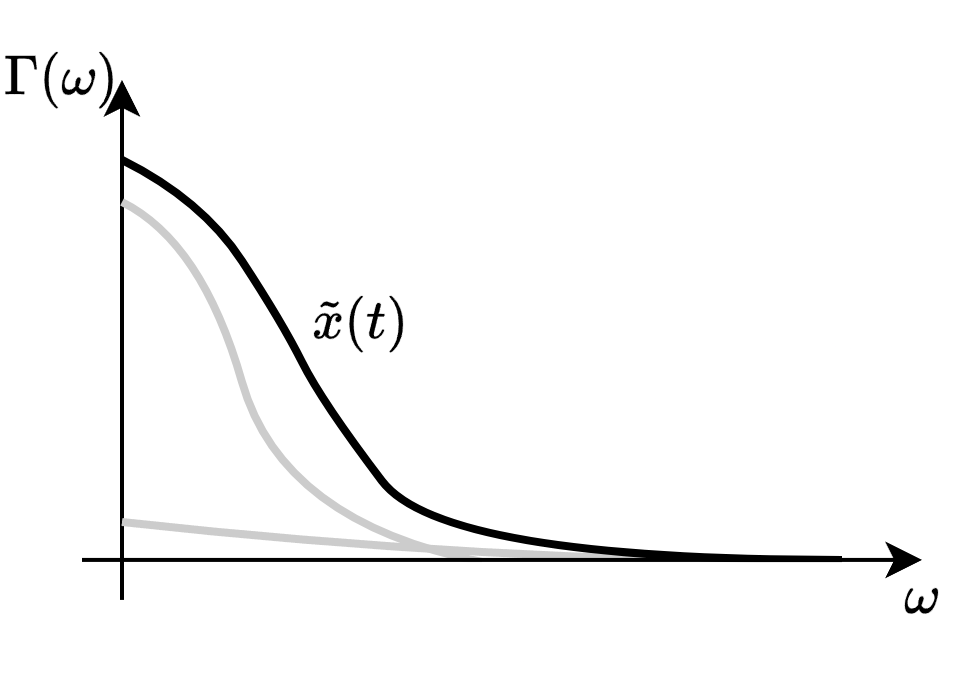
\includegraphics[width=0.4\linewidth]{images/noise.png}
    \caption{Sampled signal}
\end{figure}
The sampled signal is a combination of the true signal and noise:
\[\tilde{x}(t)=x(t)+\text{noise}\]
It's worth noting that every sampled signal has a maximum frequency content defined by the point at which the spectrum of $\tilde{x}(t)$ becomes null.

\subsection{Anti-aliasing}
Consider a sampled signal $\tilde{x}(t)$  with a null spectrum at a frequency of $2000\:Hz$. 
The dilemma arises when we desire $f_N=500\:Hz$ ($f_S=1000\:Hz$), which is significantly lower than  $2000\:Hz$. 
Direct sampling at $f_S=1000\:Hz$ violates Shannon's theorem, leading to potential aliasing problems.

\paragraph*{Analog filter}
The conventional approach to addressing this issue involves employing an analog pre-filter (anti-aliasing pre-filter).
\begin{figure}[H]
    \centering
    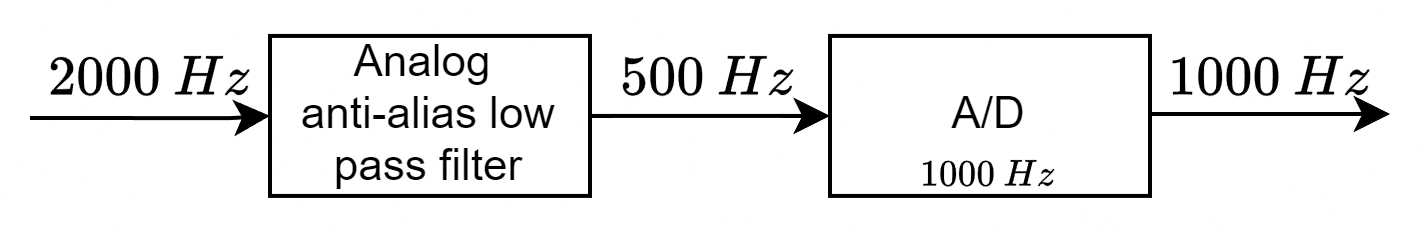
\includegraphics[width=0.7\linewidth]{images/alias.png}
    \caption{Analog filter}
\end{figure}
The output yields a discrete-time signal at $f_S=1000\:Hz$ with a maximum frequency content of $500\:Hz$, meeting the minimum requirement of Shannon's theorem.

\paragraph*{Digital filter}
Alternatively, a fully digital solution can also be utilized.
\begin{figure}[H]
    \centering
    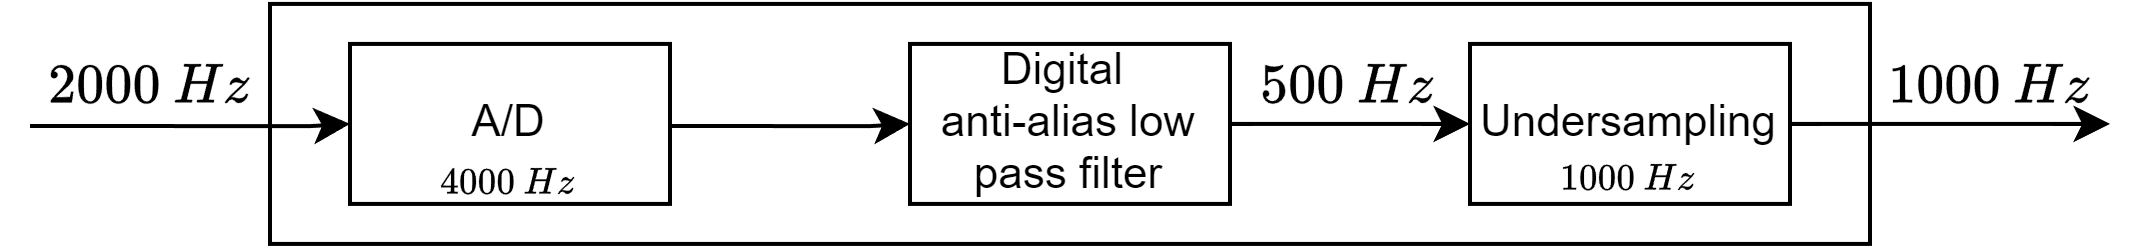
\includegraphics[width=0.9\linewidth]{images/alias1.png}
    \caption{Digital filter}
\end{figure}
This approach involves undersampling, taking one sample out of every four. 
The resulting output is a discrete-time signal at $f_S=1000\:Hz$ with a maximum frequency content of $500\:Hz$, adhering to Shannon's theorem.
The key distinction is the initial oversampling to satisfy Shannon's theorem, eliminating the necessity for an analog pre-filter.